\documentclass[acmtog]{acmart}
\usepackage{graphicx}
\usepackage{subfigure}
\usepackage{natbib}

% Title portion
\title{Assignment 4 : Ray Tracing with Global Illumination} 
\author{Student Name: Zhanrui Zhang \quad Student No. 2019533227\\ \quad Email: zhangzhr2@shanghaitech.edu.cn}

% Document starts
\begin{document}
\maketitle

\vspace*{2 ex}


\section{Introduction}

In this assignment, we are required to implement the path tracing using Monte-Carlo integration. To achieve this goal, an efficient ray-mesh intersection algorithm is implemented, as well as three different kind of BRDFs, idea diffusion, idea specular and idea transmission.

\section{Implementation Details}
\subsection{Ray Triangle Intersection}
To calculate ray-mesh intersection, we need to calculate the intersection between a ray and a single triangle. Here Möller-Trumbore algorithm is used.

The triangle is specified by three vertices, $V_1, V_2,V_3$. and the intersection point is $P$. $P$ can be represented by barycentric coordinates. Let $P = \alpha V_1 + \beta V_2 + (1-\alpha - \beta) V_3$, where $\alpha, \beta \in [0,1]$. For the ray, we can represent it with $O + tD$, where $O$ is the origin point and $D$ is the direction of ray.

Now we need to solve
\[O + tD = \alpha V_1 + \beta V_2 + (1-\alpha - \beta) V_3\]
we have three unknowns, $t$, $\alpha$ and $\beta$. After some simplification, we obtain:
\[
    \left[\begin{array}{c}
      t \\  \alpha \\ \beta
    \end{array}\right] = 
    \frac{1}{(D\times E_2)\cdot E_1}
    \left[\begin{array}{c}
        (T\times E_1) \cdot E_2\\
        (D\times E_2) \cdot T \\
        (T\times E_1) \cdot D\\
    \end{array}\right]
\]
where $T=O-V_1$, $E_1 = V_2-V_1$, $E_2 = V_3 - V_1$.

\subsection{Acceleration Structure: Uniform Grid}
Now we can calculate ray mesh intersection by calculate intersection with each triangle. However this can be extremely inefficient when there are lots of triangles. To accelerate this process, we need to construct uniform grid.

The bounding box of an object is separate into girds. If a ray hits the bounding box of the mesh object, we only tests intersection with those triangles in the gird that on the path of ray.

First we need to add all triangles of a mesh object into corresponding cells of the uniform grid. We need to loop through all triangles, find its range on x, y and z axis, and it to all cells that is covered in its x, y, z range.

Then for a given ray, we need to find which cells intersects with the ray. First we need to figure out which cell the ray starts. if the ray's origin is inside the uniform gird, we just take the cell its origin located in. If the ray's origin is outside of the uniform gird, we take the ray's intersection point with the bounding box as its reference origin and take adjacent cell as staring cell. Then we need to decide which direction the ray is marching towards.

Then we need to calculate how long the ray will march into the next grid in x, y and z direction. each time we take the closest one and add the cell index by one in that direction. Repeat the process until the ray goes out of the bounding box.

When testing ray cell intersection, we test all triangles in that cell and pic the closest intersection point. Pay attention that we need to guarantee that the intersection point is exactly in current gird since one triangle may be contained in multiple cells.

\subsection{Path Tracing with Monte-Carlo Integration}
\[L(\omega_o, p) = \int_{H^2} L(\omega_i, p) f(\omega_i, \omega_o, p) \vec{n}\cdot \vec{\omega_i} \mathrm{d}\omega_i\]
We render the image based on LTE.
\[L(\omega_o, p) = \frac{1}{N} \sum \frac{L(\omega_i, p) f(\omega_i, \omega_o, p) \vec{n}\cdot \vec{\omega_i}}{p(w_i)}\]

\subsubsection{IdeaDiffusion BRDF}
For a given cameara ray, we first need to sample a reflection direction.
For idea diffusion, we use cos-weighted method to sample the reflection direction direction. First we need to sample the direction in local coordinate. We start by uniformly sampling the unit disk.
\[r = \sqrt{\xi_1}\]
\[\theta = 2\pi \xi_2\]
where $\xi_1$ and $\xi_2$ are uniformly distributed in $(0,1)$. Then we project the point on disk to the hemsphere. So
\[x = r \cos \theta\]
\[y = r \sin \theta\]
\[z = \sqrt{1 - r^2}\]
Then we transform the local coordinate to world coordinate. Here we just use the given function in Eigen library.

Meanwhile, we can calculate the Pdf value for sampled direction. We require $p(\omega) \propto \cos \theta$.
\[
  \int_{H^2} c\cdot \cos \theta \mathrm{d}\omega = 1
\]
So for idea diffusion, $p(\omega) = \frac{\cos \theta}{\pi} = \frac{\sqrt{1-r^2}}{\pi}$

Then we need to calculate the $f$ term. For idea diffusion, the energy is distributed evenly in all direction, considering the conservation of energy, $f = \frac{1}{2\pi} \cdot C$, where $C$ is the color of object.

\subsubsection{IdeaSpecular BRDF}
For idea specular reflection, the sampled reflection direction should be the idea reflecction direction. So the sampled pdf should be 1.

\subsubsection{Light Sampling}
We can also sample the light source instead of brdf.
\[L(\omega_o, p) = \int_{H^2} L(\omega_i, p) f(\omega_i, \omega_o, p) \vec{n}\cdot \vec{\omega_i} \frac{\cos \theta'}{||x'-x||^2} \mathrm{d}A\]
Where $\cos \theta'$ is the dot product of light normal and sampled ray direction. $||x'-x||^2$ is the squre of the distance of sampled point on light source and current point.

Sampling an area light is quite simple, we only need to sample through two edges' direction to get the position of sampled point. And the pdf returned should be $\frac{1}{A}$, where $A$ is the area of light source.

\subsubsection{Direct and Indirect Lighting}
To calculate indirect light, we sample a new directoin based on object's brdf can construct a new ray. Then we test if the ray hits the light, if it does not hit the light, it means this ray is not a direct lighting ray. Then we recursively calucate the radiance based on this new ray.

For direct lighting, we sample the light source to construct a new ray, if the new ray is not blocked by other object, we use the emission of light source as $L_i$ term.

\subsubsection{Multiple Importance sampling}
For idea specular brdf, since all reflection is highly concentrated on the same direction, sampling on light source becomes inefficient. So we need to use multiple importance sampling. The basic idea is to sample with different strategy, and then combine them together with different weight.
Here power huresitc is used.
\[w_s = \frac{p_s^2}{\sum_i p_i^2}\]

After considering two different sampling strategy we can get a better result. However, for specular and diffusion material, introduce another sampling strategy would cause larger variance, so the result could be more noisy that original one. But the direct ligthing part on specular material is much better than before.

\section{Results}

For the diffusion part, the result is as follow (with different light setting)
\begin{figure}[h]
  \centering
  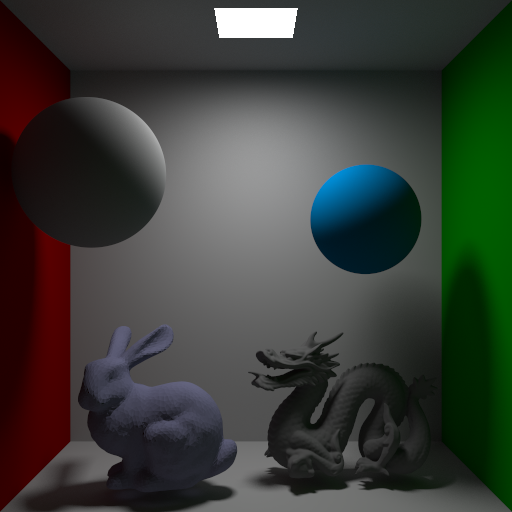
\includegraphics[scale=0.35]{images/all_diff_1.png}

  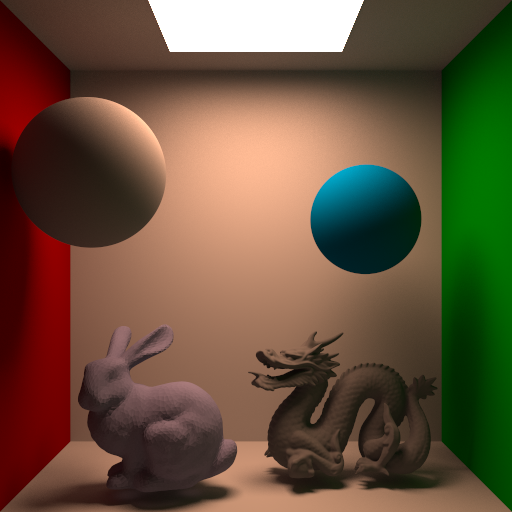
\includegraphics[scale=0.35]{images/diff_2048_2_final.png}
  \caption{Idea Diffusion}
\end{figure}

For specular, the result is similar, for save time, the dragon model is not included in this figure.
\begin{figure}[h]
  \centering
  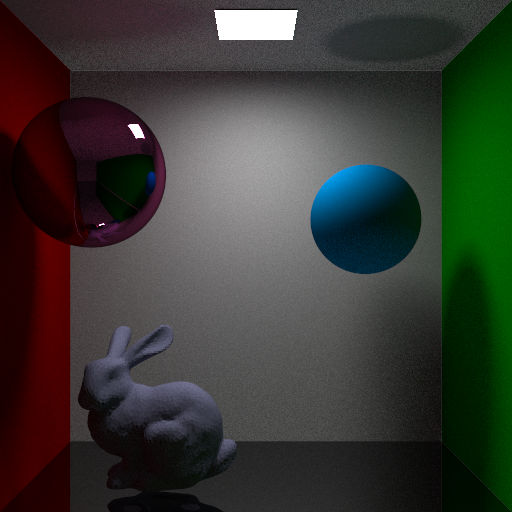
\includegraphics[scale=0.35]{images/spec_mis_4096.png}
  \caption{Set2}
\end{figure}


\end{document}
